% !TEX spellcheck = en-US
\chapter{Introduction}
\label{cha:introduction} 
In this tutorial, we discuss the topic of position and orientation estimation using inertial sensors. We consider two separate problem formulations. The first is estimation of orientation only, while the other is the combined estimation of both position and orientation. The latter is sometimes called \textit{pose estimation}. We start by providing a brief background and motivation in \Sectionref{sec:intro-background} and explain what inertial sensors are and give a few concrete examples of relevant application areas of pose estimation using inertial sensors. In \Sectionref{sec:intro-imusForPose}, we subsequently discuss how inertial sensors can be used to provide position and orientation information. Finally, in \Sectionref{sec:intro-outline} we provide an overview of the contents of this tutorial as well as an outline of subsequent chapters. 

\section{Background and motivation}
\label{sec:intro-background}
The term \textit{inertial sensor} is used to denote the combination of a three-axis accelerometer and a three-axis gyroscope. Devices containing these sensors are commonly referred to as \glspl{imu}. Inertial sensors are nowadays also present in most modern smartphone, and in devices such as Wii controllers and \gls{vr} headsets, as shown in \Figureref{fig:intro-inertialSensors}. 

\begin{figure}
  \centering
    \subfigure[Left bottom: an Xsens MTx \gls{imu}~\citep{xsens-tutorial}. Left top: a Trivisio Colibri Wireless \gls{imu}~\citep{trivisio-tutorial}. Right: a Samsung Galaxy S4 mini smartphone.]{
  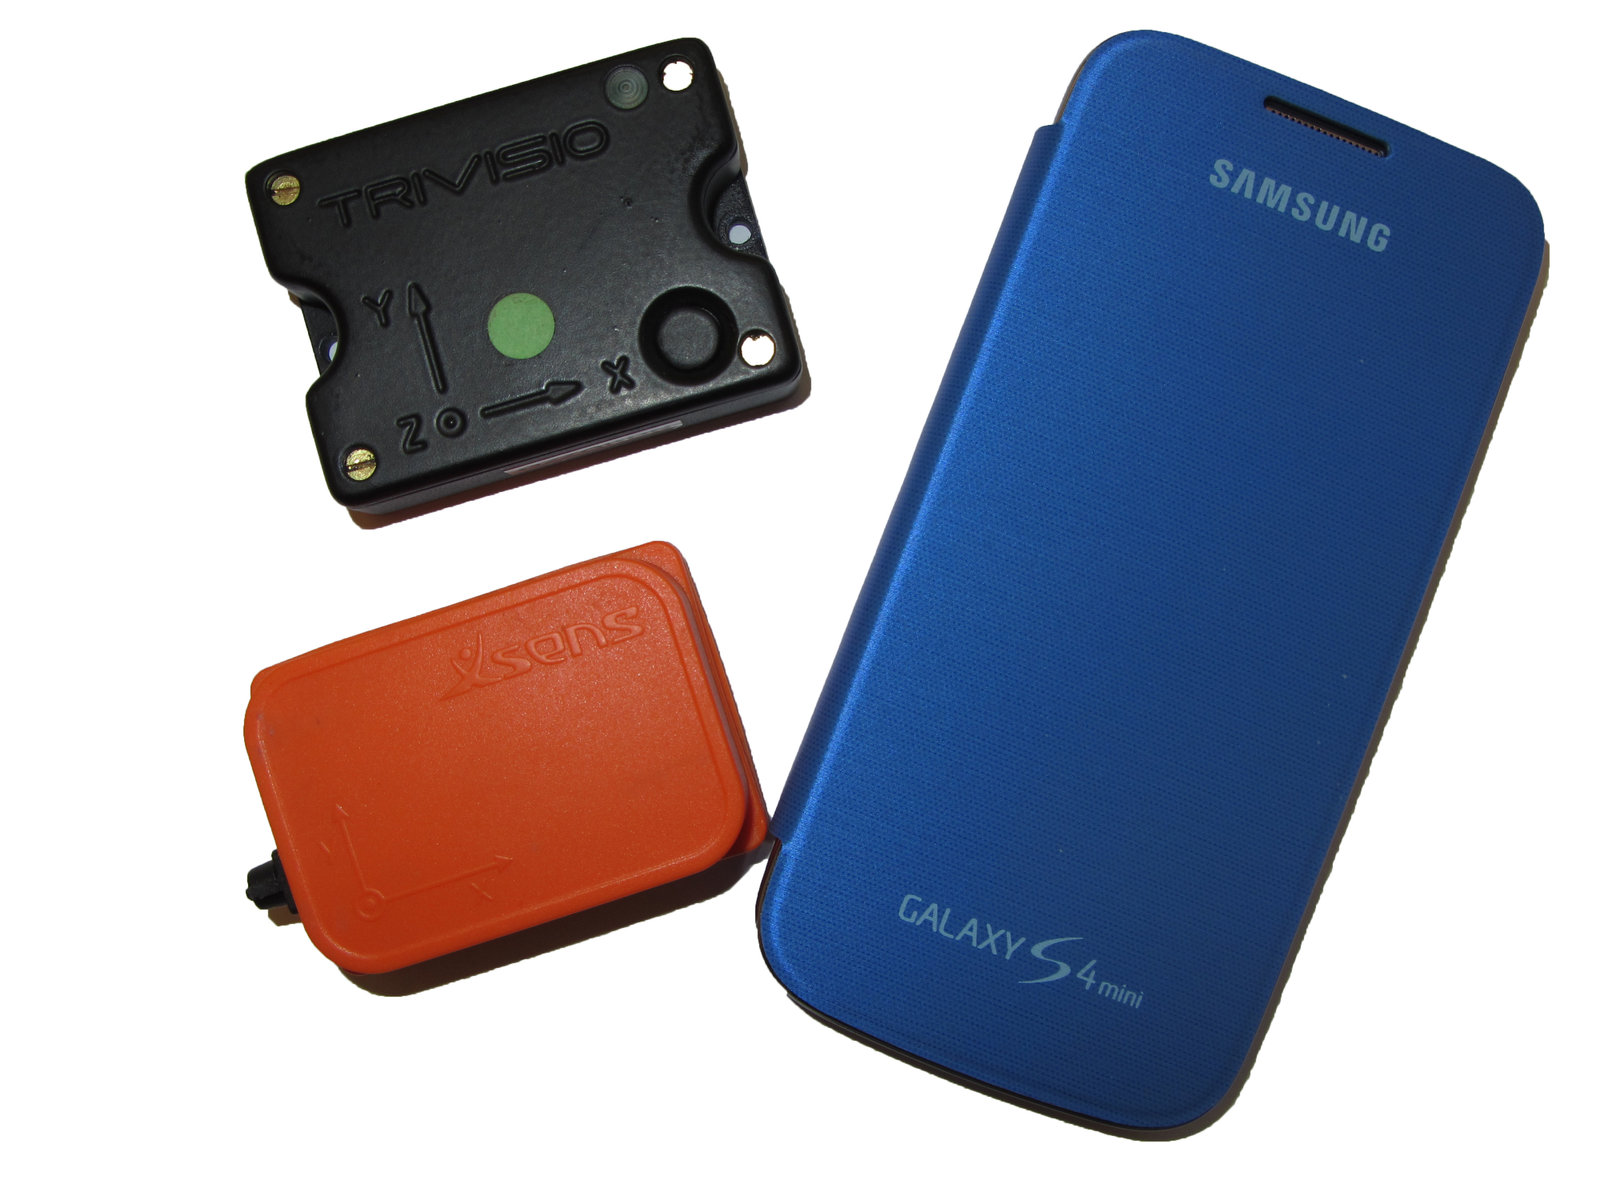
\includegraphics[height = 0.35\textwidth]{figure1_1a}} \\
  \subfigure[A Samsung gear \gls{vr}.$^1$ ]{
  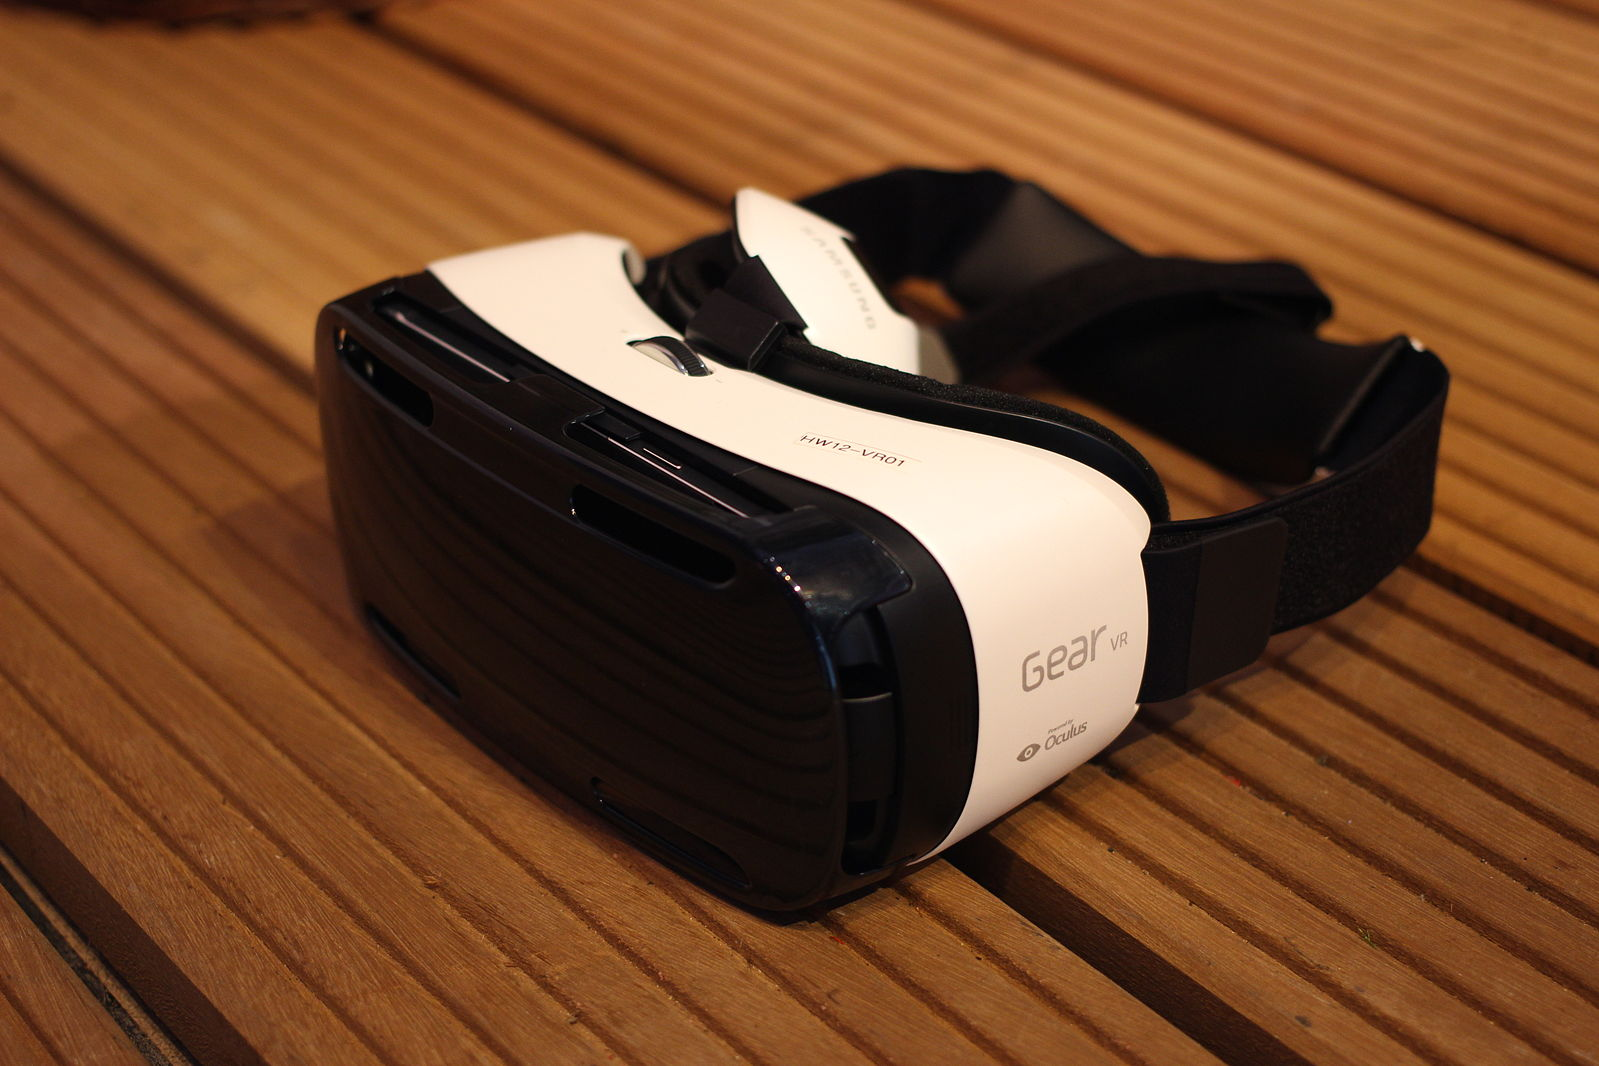
\includegraphics[height = 0.3\textwidth]{figure1_1b}} \hspace{3mm}
    \subfigure[A Wii controller containing an accelerometer and a MotionPlus expansion device containing a gyroscope.$^2$]{
  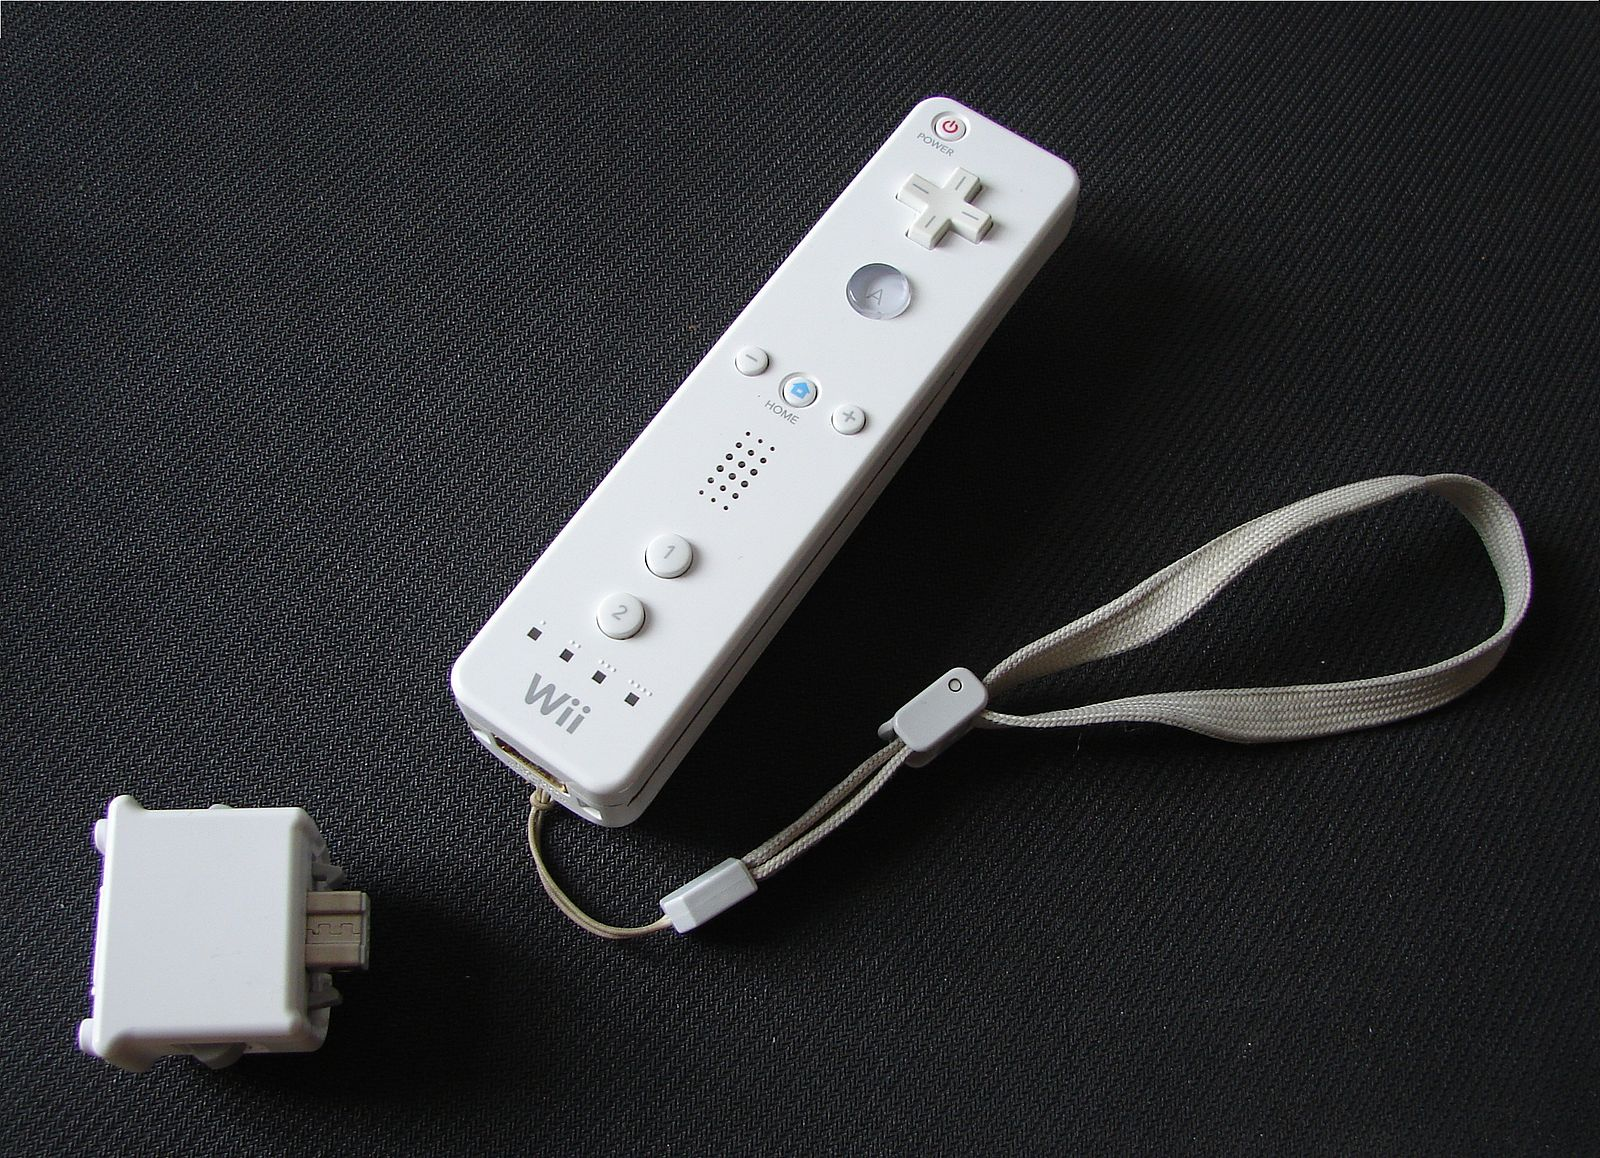
\includegraphics[height = 0.3\textwidth]{figure1_1c}}
  \caption{Examples of devices containing inertial sensors.}
  \vspace{2cm} 
  \footnoterule
  \vspace{-0.3cm}
  \flushleft \setlength{\rightskip}{0pt} 
  \footnotesize{\hspace{1em} $^1$ `Samsung Gear \gls{vr}'  available at \url{flic.kr/photos/pestoverde/15247458515} under CC BY 2.0 (\url{http://creativecommons.org/licenses/by/2.0}).}
  
  \footnotesize{\hspace{1em} $^2$ `WiiMote with MotionPlus' \hspace{0.3pt} by \hspace{0.3pt} Asmodai \hspace{0.3pt} available \hspace{0.3pt} at \hspace{0.3pt} \url{https://commons.wikimedia.org/wiki/File:WiiMote_with_MotionPlus.JPG} under CC BY SA (\url{https://creativecommons.org/licenses/by-sa/3.0/}).}
  \label{fig:intro-inertialSensors}
\end{figure}

\setcounter{footnote}{2}

A gyroscope measures the sensor's \emph{angular velocity}, \ie the rate of change of the sensor's orientation. An accelerometer measures the \emph{external specific force} acting on the sensor. The specific force consists of both the \emph{sensor's acceleration} and the \emph{earth's gravity}. Nowadays, many gyroscopes and accelerometers are based on \gls{mems} technology. \Gls{mems} components are small, light, inexpensive, have low power consumption and short start-up times. Their accuracy has significantly increased over the years. 

There is a large and ever-growing number of application areas for inertial sensors, see \eg \cite{barbourS:2001,hol:2011,perlmutterR:2012,xsens-tutorial}. Generally speaking, inertial sensors can be used to provide information about the pose of any object that they are rigidly attached to. It is also possible to combine multiple inertial sensors to obtain information about the pose of separate connected objects. Hence, inertial sensors can be used to track human motion as illustrated in \Figureref{fig:intro-motionCaptureApplications}. This is often referred to as motion capture. The application areas are as diverse as robotics, biomechanical analysis and motion capture for the movie and gaming industries. In fact, the use of inertial sensors for pose estimation is now common practice in for instance robotics and human motion tracking, see \eg \cite{luingeV2005,harle:2013,raibertBNPT:2008}. A recent survey~\citep{adlerSWK:2015} shows that 28\% of the contributions to the IEEE International Conference on Indoor Positioning and Indoor Navigation (IPIN) make use of inertial sensors. Inertial sensors are also frequently used for pose estimation of cars, boats, trains and aerial vehicles, see \eg \cite{skogH:2009,chaoCC:2010}. Examples of this are shown in \Figureref{fig:intro-singleSensorApplications}. 

\begin{figure}
  \centering
  \subfigure[Back pain therapy using serious gaming. \Glspl{imu} are placed on the 
chest-bone and on the pelvis to estimate the movement of the upper body 
and pelvis. This movement is used to control a robot in the game and 
promotes movements to reduce back pain.]{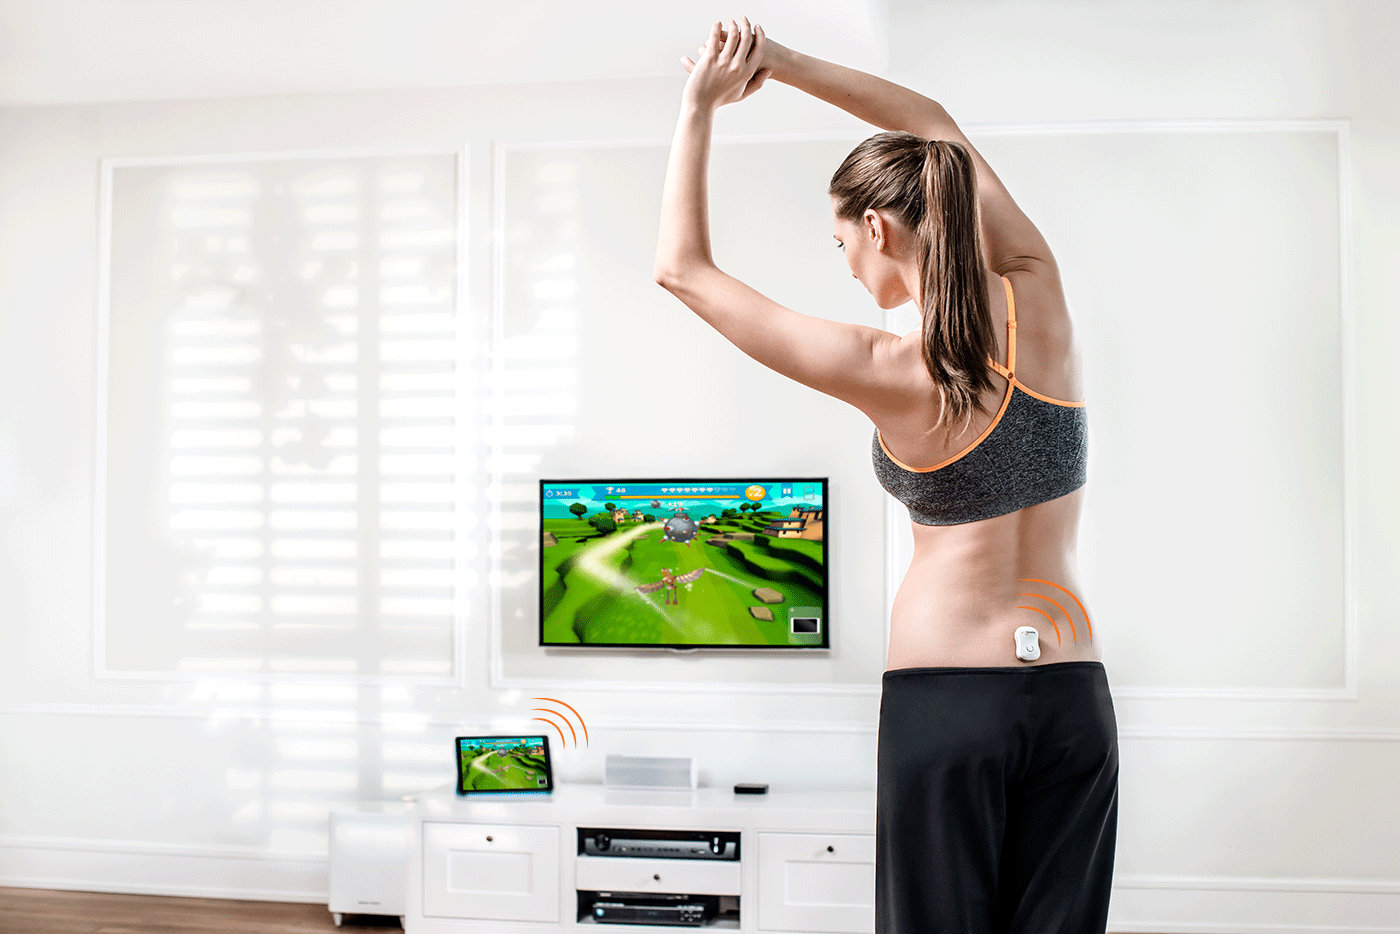
\includegraphics[height = 0.28\textwidth]{figure1_2a}} \hspace{2mm}
  \subfigure[Actor Seth MacFarlane wearing 17 \glspl{imu} to capture his motion and 
animate the teddy bear Ted. The \glspl{imu} are placed on different body segments and provide information about the relative position and orientation of each of these segments.]{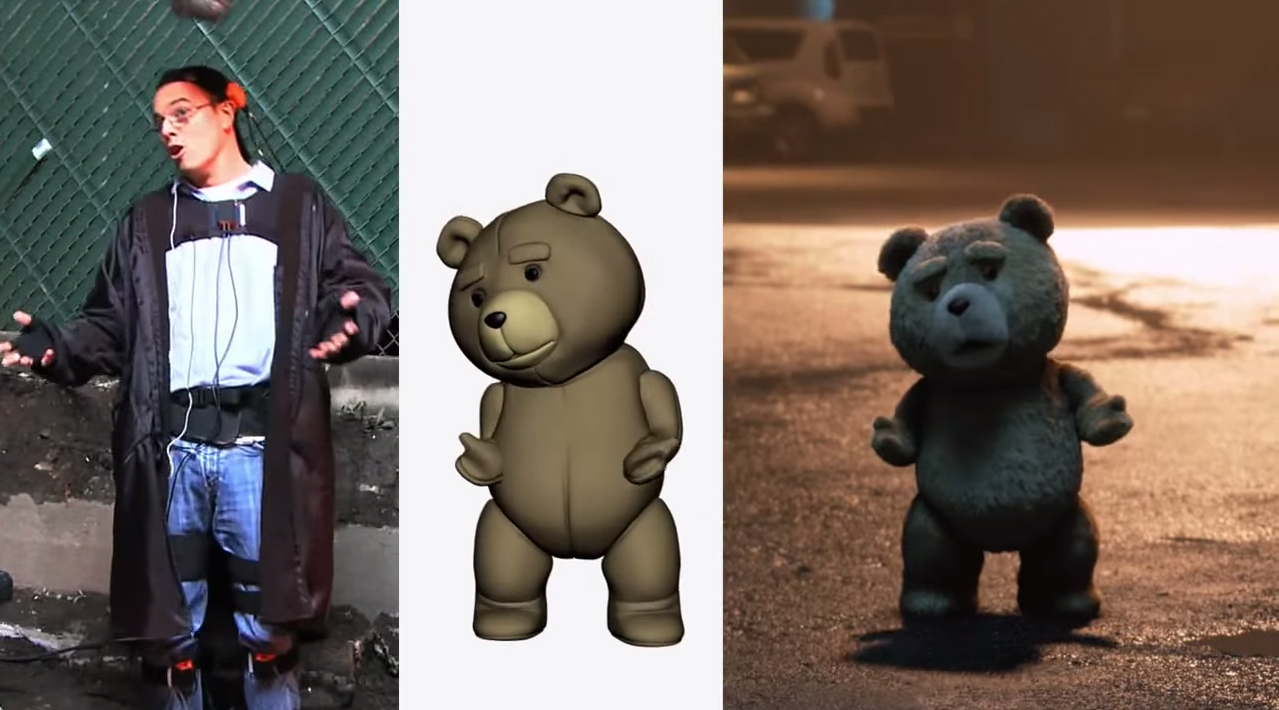
\includegraphics[height = 0.28\textwidth]{figure1_2b} \label{fig:intro-motionCaptureApplications-ted}} \\
  \caption{Examples illustrating the use of multiple \glspl{imu} placed on the 
human body to estimate its pose. Courtesy of Xsens Technologies.}
  \label{fig:intro-motionCaptureApplications}
\end{figure}

\begin{figure}
  \centering
  \subfigure[Inertial sensors are used in combination with \gls{gnss} measurements to estimate 
the position of the cars in a challenge on cooperative and autonomous 
driving.]{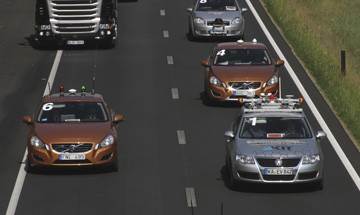
\includegraphics[height = 0.3\textwidth]{figure1_3a} } \hspace{2mm}
  \subfigure[Due to their small size and low weight, \glspl{imu} can be used to estimate the orientation for control of an unmanned helicopter.]{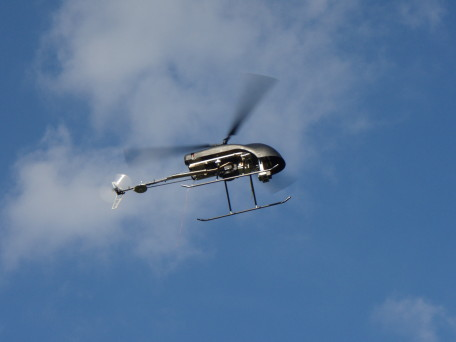
\includegraphics[height = 0.3\textwidth]{figure1_3b}}
  \caption{Examples illustrating the use of a single \gls{imu} placed on a moving 
object to estimate its pose. Courtesy of Xsens Technologies.}
  \label{fig:intro-singleSensorApplications}
\end{figure}

There exists a large amount of literature on the use of inertial sensors for position and orientation estimation. The reason for this is not only the large number of application areas. Important reasons are also that the estimation problems are nonlinear and that different parametrizations of the orientation need to be considered~\citep{grisettiKSB:2010,kurzGJH:2013}, each with its own specific properties. Interestingly, approximative and relatively simple position and orientation estimation algorithms work quite well in practice. However, careful modeling and a careful choice of algorithms do improve the accuracy of the estimates. 

In this tutorial we focus on the signal processing aspects of position and orientation estimation using inertial sensors, discussing different modeling choices and a number of important algorithms. These algorithms will provide the reader with a starting point to implement their own position and orientation estimation algorithms. 

\section{Using inertial sensors for position and orientation estimation}
\label{sec:intro-imusForPose}
As illustrated in \Sectionref{sec:intro-background}, inertial sensors are frequently used for navigation purposes where the position and the orientation of a device are of interest. Integration of the gyroscope measurements provides information about the orientation of the sensor. After subtraction of the earth's gravity, double integration of the accelerometer measurements provides information about the sensor's position. To be able to subtract the earth's gravity, the orientation of the sensor needs to be known. Hence, estimation of the sensor's position and orientation are inherently linked when it comes to inertial sensors. The process of integrating the measurements from inertial sensors to obtain position and orientation information, often called \emph{dead-reckoning}, is summarized in \Figureref{fig:intro-strapdown}.

\begin{figure}
	\centering
	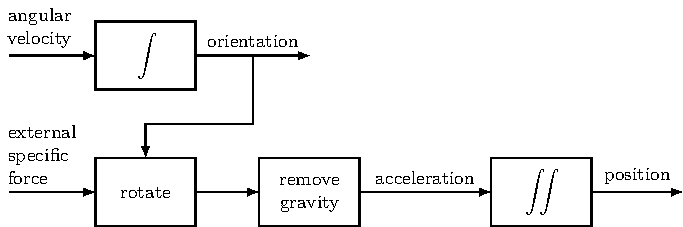
\includegraphics[scale = 1]{figure1_4.pdf}
		\caption{Schematic illustration of dead-reckoning, where the accelerometer measurements (external specific force) and the gyroscope measurements (angular velocity) are integrated to position and orientation.}
	\label{fig:intro-strapdown}
\end{figure}

If the initial pose would be known, and if perfect models for the inertial sensor measurements would exist, the process illustrated in \Figureref{fig:intro-strapdown} would lead to perfect pose estimates. In practice, however, the inertial measurements are noisy and biased as will be discussed in more detail in \Sectionref{sec:sensors-errors}. Because of this, the integration steps from angular velocity to rotation and from acceleration to position introduce \textit{integration drift}. This is illustrated in \Exampleref{ex:intro-integrationDrift}. 

\begin{myexample}{Integration drift}%
\label{ex:intro-integrationDrift}%
Let us first focus on the general case of measuring a quantity that is constant and equal to zero. The integrated and double integrated signals are therefore also equal to zero. However, let us now assume that we measure this quantity using a non-perfect sensor. In case our measurements are corrupted by a constant bias, integration of these measurements will lead to a signal which grows linearly with time. Double integration leads to a signal that instead grows quadratically with time. If the sensor instead measures a zero-mean white noise signal, the expected value of the integrated measurements would be zero, but the variance would grow with time. This is illustrated in \Figureref{fig:intro-integrationDrift} for the integration of a signal $y_t = e_t$ with $e_t \sim \mathcal{N}(0,1)$. Hence, integration drift is both due to integration of a constant bias and due to integration of noise. 

\begin{figure}
	\centering
	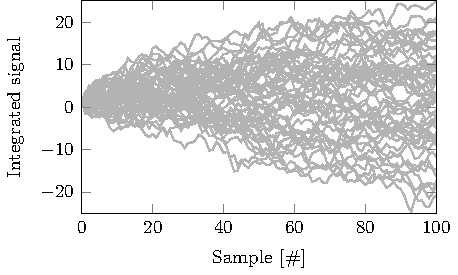
\includegraphics[scale = 1]{figure1_5.pdf}
    	\caption{Integration of a white noise signal $y_t \sim \mathcal{N}(0,1)$ for $50$ noise realizations.}
	\label{fig:intro-integrationDrift}
\end{figure}

To illustrate integration drift using experimental data, a stationary data set is collected with a Sony Xperia Z5 Compact smartphone using the app described in \cite{hendebyGWG:2017}. The smartphone contains accelerometers and gyroscopes produced by Invensense~\citep{invensense-tutorial}. We integrate the inertial measurements to obtain position and orientation estimates. Since the smartphone is kept stationary during the data collection, we expect the position and orientation to remain the same. However, the orientation estimates drift a few degrees over $10$ seconds as shown in \Figureref{fig:intro-oriDrift}. Note that the integration drift is not the same for all axes. This is mainly due to a different sensor bias in the different axes. This will be studied further in \Exampleref{ex:sensors-inertialMeasurements}, where the same data set is used to study the sensor characteristics. As shown in \Figureref{fig:intro-posDrift}, the position drifts several meters over $10 \second$. The reason for this is two-fold. First, the accelerometer measurements need to be integrated twice. Second, the orientation estimates need to be used to subtract the gravity and any errors in this will result in \emph{leakage of gravity} into the other components. 
\begin{figure}[t]
	\centering
	\subfigure[Integrated orientation for the position in $x$- (blue), $y$- (green) and $z$-direction (red).]{
	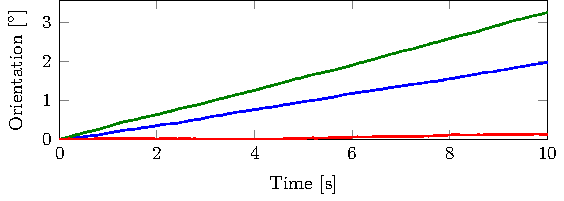
\includegraphics[scale = 1]{figure1_6a.pdf}
	\label{fig:intro-oriDrift}}
	\subfigure[Integrated position for rotation around the $x$-axis (blue), the $y$-axis (green) and the $z$-axis (red).]{
	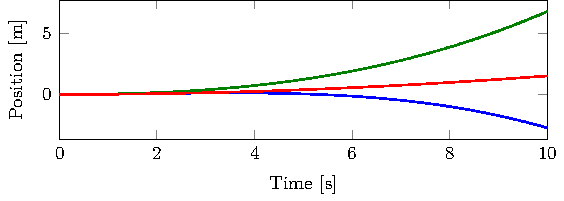
\includegraphics[scale = 1]{figure1_6b.pdf}
	\label{fig:intro-posDrift}}
	\caption{Position and orientation estimates based on dead-reckoning of the inertial sensors only. The data is collected with a Sony Xperia Z5 Compact smartphone that is lying stationary on a table.}
\end{figure}
\end{myexample}

From the example above, it can be concluded that errors in the measurements have a large impact on the quality of the estimated position and orientation using inertial sensors only. This is particularly the case for position, which relies both on double integration of the acceleration and on accurate orientation estimates to subtract the earth's gravity. Because of this, inertial sensors need to be supplemented with other sensors and other models to obtain accurate position and orientation estimates. 

Inertial sensors provide pose estimates at high sampling rates which are accurate on a short time scale but drift over longer time scales. They are therefore very suitable for being combined with sensors with a lower sampling rate but with information that does not drift over time. For pose estimation, inertial sensors are often combined with measurements from for instance a \acrfull{gnss} \citep{kaplanH:1996,tittertonW:1997,hol:2011}, an \gls{uwb} system \citep{kokHS:2015,sczysloSGK:2008,pittetRMK:2008,corralesCT:2008,deAngelisNSHC:2010} or cameras \citep{corkeLD:2007,holSLSG:2007,liM:2013,martinelli:2012}. For orientation estimation, they are often used in combination with magnetometers, which measure the direction of the magnetic field \citep{sabatini:2006,roetenbergLBV:2005}. 

This tutorial aims at giving an introduction on how to use inertial sensors for position and orientation estimation, but also on how to combine them with additional information. These additional sensors are not the focus of this paper but simple models will be used for magnetometers and sensors providing position information to illustrate the combined use of these sensors.

\section{Tutorial content and its outline}
\label{sec:intro-outline}
To obtain accurate position and orientation estimates using inertial sensors in combination with additional measurements and models, a number of important things need to be considered. First, the quantities measured by the inertial sensors need to be accurately described and the sources of error need to be characterized. This is the topic of \Chapterref{cha:sensors}. Note that throughout the tutorial, we will focus on \gls{mems} inertial sensors and consider both data from standalone \glspl{imu} and from smartphones. This implies that we do not focus on for instance mechanical or optical gyroscopes and on mechanical or solid-state accelerometers~\citep{tittertonW:1997}. These sensors may have characteristics that are quite different from the \gls{mems} inertial sensors considered here. 

Based on the analysis of the sensors in \Chapterref{cha:sensors} and on additional analysis of the application at hand, models can be constructed. This is the topic of \Chapterref{cha:models}, where we will also discuss different parametrizations of orientation. This will highlight the challenges in parametrizing and estimating orientations and show that the orientation estimation problem is inherently nonlinear. Furthermore, we will present two models that can be used for position and orientation estimation. The first is a model for pose estimation using inertial measurements in combination with position measurements. The second is a model for orientation estimation, using inertial and magnetometer measurements. 

In \Chapterref{cha:orientationEstimation}, different algorithms for position and orientation estimation will be introduced. The general structure of the algorithms will be discussed, after which explicit algorithms for orientation estimation using inertial and magnetometer measurements are given. We will also discuss how the algorithms can be extended to pose estimation when position measurements are available. Some general characteristics of the two estimation problems will be given and the quality of the estimates from the different algorithms will be analyzed. Which algorithm is most suitable for which application depends strongly on the computational power that is available, the accuracy that is required and the characteristics of the problem at hand. 

In \Chapterref{cha:orientationEstimation}, we assume that the sensors are properly calibrated. However, calibration of the sensors is important to for instance estimate the inertial sensor biases. Furthermore, calibration is specifically of concern when combining inertial data with other sensors. In these cases, it is important that the inertial sensor axes and the axes of the additional sensors are aligned. Sensor calibration is the topic of \Chapterref{cha:calibration}. As an illustrative example, we will consider the estimation of an unknown gyroscope bias. 

Our focus in this tutorial is to present models and algorithms that can be used for position and orientation estimation using inertial measurements. Because of this, we assume fairly simple models for the additional information --- the magnetometer and position measurements. In \Chapterref{cha:applications}, we will discuss how the algorithms from \Chapterref{cha:orientationEstimation} can be used in more complex settings. For example, we will consider the cases of more complex position information in the form of images from a camera, the presence of non-Gaussian measurement noise and the availability of additional information that can be exploited. The information provided by the inertial sensors remains one of the main building blocks of algorithms that can be used for these cases. Adaptations of the algorithms presented in \Chapterref{cha:orientationEstimation} can therefore be used to also solve these more complex scenarios. We will end this tutorial with some concluding remarks in \Chapterref{cha:conclusions}.